% !Tex root = Vorlage.tex
\section{Experiments}
To examine robustness as it is defined in the previous chapter, a number of experiments are conducted.
Then, in order to evaluate the capabilities of ERM-techniques for FD discovery, the DepDetector algorithm is run on a number of datasets.
For the experiments, datasets from the UCI Machine Learning Repository are used.~\cite{DUA19}

Since the algorithms analyzed in this section handle missing values differently, rows containing missing values are excluded from the datasets due to possible inconsistencies when comparing results.

\subsection{FD Imputer}
FD Imputer is run for every FD found on a train set of a dataset.
The measured performance-score is called robustness of the FD.
First, experiments on the imputation of classifiable data with the FD Imputer are presented.
Then, results obtained when imputing continuous data are discussed.

\begin{figure}[ht]
     \centering
     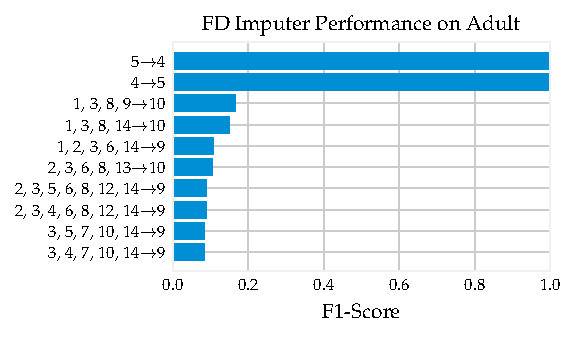
\includegraphics[width=\textwidth]{../figures/adult/f1_fd_imputer.pdf}
     \caption{F1-Scores of the seven most-robust FDs on the Adult dataset when imputing classifiable values.}
     \label{fig:f1_fd_adult}
\end{figure}

\subsubsection{Imputation of Classifiable Data}
Figure~\ref{fig:f1_fd_adult} shows the performance of FD Imputer on the Adult dataset.
The two top performing FDs have a perfect F1-Score of 1 each.
An explanation for this circumstance can be found when analyzing the content of columns 4 and 5.

Column 4 contains information about the highest educational level achieved.
There are 16 different categories of educational level defined.
Each category is assigned an integer in a range spanning from 0 to 15.
This integer is the content of column 5.
Thus, the relation between column 4 and column 5 can be modeled by a bijective function, projecting the domains of each attribute onto the other.
In consequence, FDs between column 4 and 5 are perfectly robust.

All other FDs found on the Adult dataset lead to F1-Scores smaller than \( 0.2\), being substantially less robust than the two top-performing FDs.
It can be derived that only the two top-performing FDs can be used to meaningfully impute data.
If new data was added to the dataset, it can thus safely be assumed that these two FDs still held.
In reverse, no value in a column other than 4 or 5 can be meaningfully imputed using FDs detected on the Adult dataset due to the small robustness of these FDs.
\begin{figure}[ht]
     \centering
     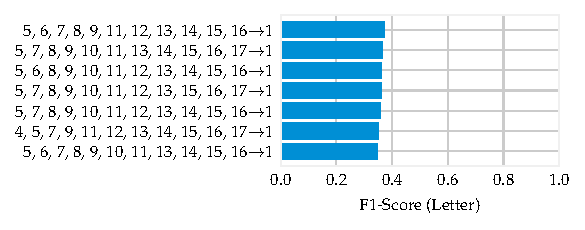
\includegraphics[width=\textwidth]{../figures/letter/f1_fd_imputer.pdf}
     \caption{Robustness of the seven top-performing FDs on the Letter dataset when imputing classifiable RHSs.}
     \label{fig:f1_fd_letter}
\end{figure}
Figure~\ref{fig:f1_fd_letter} displays the result of running FD Imputer on the Letter dataset.
Of the 80 FDs found on the train split, the seven most robust ones share the same RHS, column 1.
No F1-Score greater than 0.37 is achieved on this dataset.

All analyzed datasets other than Adult yield no FD with a perfect score.
Only an FD on the Breast Cancer Wisconsin dataset achieves a score higher than 0.75.
Table~\ref{tab:fd-imputer-performance} provides a summary of how FD Imputer performs on eight different datasets.

In Table~\ref{tab:fd-imputer-performance}, Column \#FDs indicates how many FDs were found on the complete dataset.
\#FDs\textsubscript{train} contains the number of FDs that were detected on the train set.
F1\textsubscript{mean} and F1\textsubscript{max} indicate the arithmetic mean and maximal F1-Score achieved on each dataset respectively.
The last column named \#(F1 = 0) provides the number of FDs that scored a F1-Score of 0.

\begin{table}[ht]
    \centering
    \begin{tabular}{lrrrrrr}
        \toprule
        \toprule
        & & & & \multicolumn{3}{c}{Classification Performance} \\
        \cmidrule(lr{.25em}){5-7}
        Dataset & Attributes & \#FDs & \#FDs\textsubscript{train} & \#FD (F1 = 0) & F1\textsubscript{mean} & F1\textsubscript{max} \\
        \midrule
        Abalone & 10 & 175 & 193 & 45 & 0.0008 & 0.0048 \\
        Adult & 16 & 93 & 88 & 10 & 0.0669 & 1.0000 \\
        Balance S. & 6 & 7 & 7 & 6 & 0.0000 & 0.0000 \\
        Breast C. W. & 12 & 57 & 77 & 10 & 0.2198 & 0.7539 \\
        Chess & 8 & 9 & 9 & 8 & 0.0000 & 0.0000 \\
        Iris & 6 & 9 & 8 & 1 & 0.1274 & 0.2252 \\
        Letter & 18 & 78 & 80 & 17 & 0.2347 & 0.3737 \\
        Nursery & 10 & 11 & 11 & 10 & 0.0000 & 0.0000  \\
        \bottomrule
        \bottomrule
    \end{tabular}
    \caption{Performance of the FD Imputer on a selection of UCI datasets.}\label{tab:fd-imputer-performance}
\end{table}

The results displayed in table~\ref{tab:fd-imputer-performance} show that robustness depends strongly on the dataset considered.
However, no relation between \#FDs and robustness can be identified (see appendix figure~\ref{fig:robustness-number-of-classifiable-fds}).
Analysis on a bigger body of datasets seems necessary to draw further conclusions.

\subsubsection{Imputation of Continuous Data}
The majority of columns for which FDs are detected in this work contain classifiable data.
However, some FDs are found whose RHSs contains continuous data.
For brevity, we call such an FD continuous FD or \emph{cFD}.
Table~\ref{tab:fd-imputer-mse} displays an overview of how FD Imputer performs when imputing continuous RHS values.
Continuous FDs were detected on seven train sets of the eight datasets considered --- column `\# continuous FDs\textsubscript{train}' in table~\ref{tab:fd-imputer-mse} shows how many cFDs were detected.

Column `0-Coverage cFDs' displays for how many cFDs not a single imputation was found.
If all cFDs found on the train set are `0-coverage cFDs', the resulting `Coverage' is thus 0\% with missing minimum and maximum values.

The column named `Coverage' indicates the mean imputation coverage.
Mean imputation coverage is the mean percentage of rows in the test set for which imputations were found per cFD.
It was computed according to the following formula:

\begin{align*}
    \text{mean missing values per cFD} &= \sum_{i} \frac{\text{missing imputations}}{\text{cFD}_i} \cdot \left(\text{\# cFDs}\right)^{-1} \\
    \text{mean coverage} &= \left( 1 - \frac{\text{mean missing values per cFD}}{\text{\# rows in }r_{test}} \right) \cdot 100
\end{align*}

Note that the computed mean coverage is a percentage.

On the Letter dataset, no cFD is detected.
Five out of seven datasets for which cFDs were detected have a mean imputation coverage of 0\%.
Concerning the two datasets with nonzero mean imputation coverage, the mean imputation coverage is approximately one per mill.

\begin{table}[ht]
    \centering
    \begin{tabular}{lrrr}
        \toprule
        \toprule
        Dataset & \# cFDs\textsubscript{train} & \# 0-Coverage cFDs  & Coverage (\%) \\
        \midrule
        Abalone & 139 & 84 & 0.1277 \\
        Adult & 11 & 5 & 0.1217 \\
        Balance S. & 1 & 1 & 0.0000 \\
        Breast C. W. & 1 & 1 & 0.0000 \\
        Chess & 1 & 1 & 0.0000 \\
        Iris & 4 & 4 & 0.0000 \\
        Letter & 0 & 0 & - \\
        Nursery & 1 & 1 & 0.0000 \\
        \bottomrule
        \bottomrule
    \end{tabular}
    \caption{Imputation coverage of FD Imputer on all UCI datasets for which FDs with continuous data in the RHS were detected.}\label{tab:fd-imputer-mse}
\end{table}

Since the MSE is an absolute error measure, comparisons between cFDs concerning different RHSs do not provide any insights.
Table~\ref{tab:fd-imputer-mse-abalone} gives an overview of all cFDs examined on the Abalone dataset.
Mind that every cFD that is used by FD Imputer to return imputations yields exactly one MSE.

Column `RHS' indicates the RHS, for which cFDs were examined.
The next column `Var(MSE)' contains the experimental variance of the mean MSE.
The latter is called \( \overline{\text{MSE}} \) and is displayed in the following column.
The last two columns `MSE\textsubscript{min}' and `MSE\textsubscript{max}' contain the minimum and maximum MSEs.

From the eight RHSs displayed in table~\ref{tab:fd-imputer-mse-abalone}, six RHSs show similar statistical results.
For these six RHSs, the variance of MSEs is very small and lies between \( 10^{-7} \) and \( 10^{-9} \).
In addition, the mean MSEs are distributed within two orders of magnitude, the maximum MSE within one order of magnitude.

All values observed for RHS 0 are between \( 10^{5} \) and \( 10^{21} \) bigger than values observed for other RHSs.
Column 0 of the Abalone dataset contains the row-ID.
Since there is no dependency between any column-combination in the dataset and the row-ID, a high MSE seems plausible.

\begin{table}[ht]
    \centering
    \begin{tabular}{lrrrr}
        \toprule
        \toprule
        RHS & Var(MSE) & \( \overline{\text{MSE}} \) & MSE\textsubscript{min} & MSE\textsubscript{max} \\
        \midrule
        0 & \( 2.0712 \cdot 10^{13} \) & \( 7.9385 \cdot 10^{6} \) & \( 8.2705 \cdot 10^{5} \) & \( 1.3418 \cdot 10^{7} \) \\
        2 & \( 1.3039 \cdot 10^{-7} \) & \( 2.3393 \cdot 10^{-4} \) & 0.0000 & \( 9.2500 \cdot 10^{-4} \) \\
        3 & \( 3.5634 \cdot 10^{-7} \) & \( 3.5412 \cdot 10^{-5} \) & 0.0000 & \( 1.6250 \cdot 10^{-4} \) \\
        4 & \( 3.4298 \cdot 10^{-9} \) & \( 2.0972 \cdot 10^{-4} \) & \( 1.1250 \cdot 10^{-4} \) & \( 3.1250 \cdot 10^{-4} \) \\
        5 & \( 3.0624 \cdot 10^{-9} \) & \( 6.9775 \cdot 10^{-5} \) & \( 9.0000 \cdot 10^{-6} \) & \( 1.6700 \cdot 10^{-4} \) \\
        6 & \( 2.2867 \cdot 10^{-9} \) & \( 1.5017 \cdot 10^{-4} \) & \( 8.4500 \cdot 10^{-5} \) & \( 1.9700 \cdot 10^{-4} \) \\
        7 & 0.0000 & 0.0000 & 0.0000 & 0.0000 \\
        8 & \( 7.4015 \cdot 10^{-9} \) & \( 1.0366 \cdot 10^{-4} \) & 0.0000 & \( 2.2250 \cdot 10^{-4} \) \\
        \bottomrule
        \bottomrule
    \end{tabular}
    \caption{Statistical analysis of the computed MSEs when running FD Imputer with 84 different cFDs on the Abalone dataset.}\label{tab:fd-imputer-mse-abalone}
\end{table}

If column 7 of the Abalone dataset is imputed with cFDs, the task results in a perfect MSE of 0.
On closer inspection, column 7 is the RHS of eleven cFDs.
Only one of those eleven cFDs can be used by FD Imputer to impute exactly one value --- which happens to be an exact match.

Half of the RHSs are determined by at least one cFD with a perfect MSE of 0.
This shows that perfect imputations are common when running FD Imputer with cFDs.

\subsection{ML Imputer}
ML Imputer is executed with the same set of FDs as FD Imputer.
Analogously to the discussion of experiments executed with FD Imputer, the evaluation will be separated into two sections, one discussing FDs with classifiable RHSs, the other examining FDs with continuous RHSs.

\subsubsection{Imputation of Classifiable Data}
The first dataset analyzed is Adult.
Figure~\ref{fig:f1_ml_adult} displays the F1-Scores of the seven best performing FDs.
The two top-scoring FDs are the same for FD Imputer and ML Imputer.
The third most top-performing FD is \( 0 \rightarrow 14\), a relation between row-ID and nationality.
\begin{figure}[ht]
     \centering
     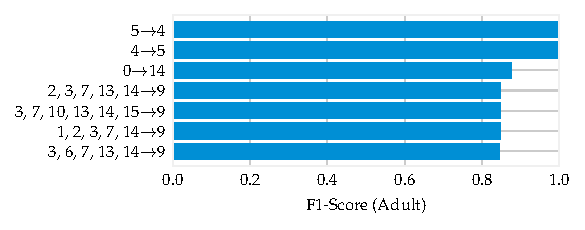
\includegraphics[width=\textwidth]{../figures/adult/f1_ml_imputer.pdf}
     \caption{The figure compares the F1-Score of the FD Imputer compared to the F1-Score of the ML Imputer. Each point represents one FD.}
     \label{fig:f1_ml_adult}
 \end{figure}
There is no apparent dependency between row-ID and nationality.
Inspecting the distribution of values in column 14, one cause for the performance of FD \( 0 \rightarrow 14 \) can be derived.
% Maybe plot histogram
Of 24154 rows in the train set, 22020 entries contain the value `United-States'.
ML Imputer learns the same imputation for all 2987 entries in the test set, namely `United-States'.
This perfectly explains the performance of FD \( 0 \rightarrow 14\).

The bar plot in figure~\ref{fig:f1-ml-imputer-chess} shows the performance of ML Imputer on the Chess dataset.
The FD with the biggest F1-Score is \( 0 \rightarrow 7 \).
Column 0 contains the row-ID, whereas column 7 contains the outcome of a chess-game, assuming both players play perfectly.
Again, there does not seem to exist a relation between the two columns.
On closer inspection however it can be observed that the Chess-dataset is sorted.
For tuples with row-ID of less than 2796, column 7 contains always the value `draw'.
Tuples that have a row-ID bigger than 2795 but smaller than 2824 always contain the value `zero' and so on.

This showcases the capabilities of ML Imputer to learn relaxation on the extent, similar to what is used in the definition of CFDs, ECFDs and CFD\textsuperscript{p}s:
ML Imputer approximately learns a pattern where a dependency \( 0 \rightarrow 7\) holds, if \( 0 \leq \text{ row-ID } \leq 2795 \) or \( 2796 \leq \text{ row-ID } \leq 2823 \), and so on.

\begin{figure}[ht]
     \centering
     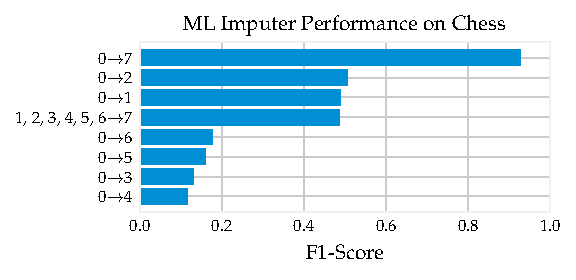
\includegraphics[width=\textwidth]{../figures/chess/f1_ml_imputer.pdf}
     \caption{F1-Scores of the seven top-performing FDs on the Adult dataset.}
     \label{fig:f1-ml-imputer-chess}
 \end{figure}

Table~\ref{tab:ml-imputer-performance} shows a generally higher performance of ML Imputer compared to FD Imputer.
There are no FDs for which ML Imputer scores 0.
This can be explained by the property of ML Imputer of always returning some imputation value, even if the probability with which ML Imputer predicts a value is low.
On the other hand there is FD Imputer, which frequently does not return any imputation value at all.

\begin{table}[ht]
    \centering
    \begin{tabular}{lrrrrr}
        \toprule
        \toprule
        & & & \multicolumn{3}{c}{Classification Performance} \\
        \cmidrule(lr{.25em}){4-6}
        Dataset & \#FDs & \#FDs\textsubscript{train} & F1\textsubscript{mean} & F1\textsubscript{max} & F1\textsubscript{min} \\
        \midrule
        Abalone & 175 & 193 & 0.3697 & 0.5664 & 0.0619 \\
        Adult & 93 & 88 & 0.7720 & 1.0000 & 0.0409 \\
        Balance Scale & 7 & 7 & 0.4670 & 0.9443 & 0.0255 \\
        Chess & 9 & 9 & 0.3744 & 0.9276 & 0.1162 \\
        Iris & 9 & 8 & 0.9243 & 1.0000 & 0.1275 \\
        Letter & 78 & 80 & 0.7207 & 0.9134 & 0.0058 \\
        Nursery & 11 & 11 & 0.9915 & 0.4531 & 0.1138 \\
        \bottomrule
        \bottomrule
    \end{tabular}
    \caption{Performance of ML Imputer on eight different datasets when training on FDs with classifiable RHS entries.}\label{tab:ml-imputer-performance}
\end{table}

\subsubsection{Imputation of Continuous Data}
When ML Imputer is run with cFDs, internally a regression is performed.
To examine how this mechanism behaves, imputation generation based on cFDs was performed.
ML Imputer always returns imputations, thus there are no missing values as listed in table~\ref{tab:fd-imputer-mse} --- ML Imputer coverage is always 100\%.

As done for the FD Imputer in table~\ref{tab:fd-imputer-mse-abalone}, an in-depth analysis is performed on the Abalone dataset in table~\ref{tab:ml-imputer-mse-abalone}.
The biggest mean MSE is returned for RHS 0, which contains the row-ID.
This can be explained with the observation that the data is neither sorted, nor are there any other dependencies between the contents of the Abalone dataset and the row-ID.

\begin{table}[ht]
    \centering
    \begin{tabular}{lrrrr}
        \toprule
        \toprule
        RHS & Var(MSE) & \( \overline{\text{MSE}} \) & MSE\textsubscript{min} & MSE\textsubscript{max} \\
        \midrule
        0 & \(3.7736 \cdot 10^{9} \) & \(1.4656 \cdot 10^{6} \) & \(1.3884 \cdot 10^{6} \) & \(1.6045 \cdot 10^{6} \) \\
        2 & \( 1.3150 \cdot 10^{-5} \) & \( 1.5828 \cdot 10^{-3} \) & \( 3.0536 \cdot 10^{-4} \) & \( 1.4630 \cdot 10^{-2} \) \\
        3 & \( 5.3958 \cdot 10^{-6} \) & \( 9.6910 \cdot 10^{-4} \) & \( 2.0273 \cdot 10^{-4} \) & \( 1.0238 \cdot 10^{-2} \) \\
        4 & \( 9.2724 \cdot 10^{-8} \) & \( 3.2361 \cdot 10^{-4} \) & \( 2.2714 \cdot 10^{-4} \) & \( 1.5399 \cdot 10^{-3} \) \\
        5 & \( 3.5212 \cdot 10^{-3} \) & \( 2.1342 \cdot 10^{-2} \) & \( 1.6185 \cdot 10^{-3} \) & \( 2.5844 \cdot 10^{-1} \) \\
        6 & \( 1.5414 \cdot 10^{-4} \) & \( 6.6988 \cdot 10^{-3} \) & \( 1.2499 \cdot 10^{-3} \) & \( 5.2755 \cdot 10^{-2} \) \\
        7 & \( 1.1345 \cdot 10^{-5} \)& \( 1.9497 \cdot 10^{-3} \) & \( 4.8120 \cdot 10^{-4} \) & \( 1.2581 \cdot 10^{-2} \) \\
        8 & \( 1.7069 \cdot 10^{-5} \) & \( 2.8521 \cdot 10^{-3} \) & \( 9.7318 \cdot 10^{-4} \) & \( 1.9730 \cdot 10^{-2} \) \\
        \bottomrule
        \bottomrule
    \end{tabular}
    \caption{Statistical analysis of the Abalone dataset obtained by running ML Imputer with the same 84 cFDs as used in the generation of table~\ref{tab:fd-imputer-mse-abalone}.}\label{tab:ml-imputer-mse-abalone}
\end{table}

All other RHSs lead to performance measures that seem plausible.
Variances are between one and four orders of magnitude smaller than the corresponding arithmetic means, minimum and maximum MSEs are separated by up to two orders of magnitude.

\subsection{Overfitting ML Imputer}
If the neural network trained by ML Imputer learns too many examples, the resulting model is just a memorization of the whole training-set --- a phenomenon referred to as overfitting.~\cite[p.~164]{HAY08}
To further investigate ML Imputer's capabilities of overfitting models, experiments are conducted to compare imputation performance between a overfitted model and a normally trained model.
Overfitting was achieved by first uniting \( r_{train} \) and \( r_{test} \) and then training and testing the model on the same unified relational instance.
Internally, this unification of train set and test set implies that the resulting train-error and test-error are the same entity, effectively preventing cross-validation.

Figure~\ref{fig:f1-ml-overfit-adult} compares an overfitted model with a cross-validated model on the Adult dataset.
Every blue data point represents one FD, providing the data with which the models were trained.
The red graph in figure~\ref{fig:f1-ml-overfit-adult} is the graph of the identity function.
All data points that lie below the graph of the identity function indicate that the overfitted model scores higher than the cross-validated model.
Data points that lie above the graph of the identity function represent the opposite.
Both models score equally well, if a data point lies on the graph of the identity function.
\begin{figure}[ht]
     \centering
     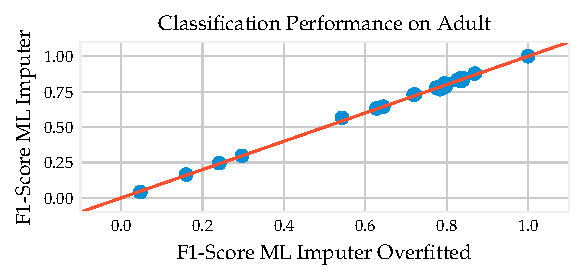
\includegraphics[width=\textwidth]{../figures/adult/f1_ml_overfit.pdf}
     \caption{Comparison of an overfitted model with a conventionally trained model on the Adult dataset.}
     \label{fig:f1-ml-overfit-adult}
\end{figure}
The distribution of data points in figure~\ref{fig:f1-ml-overfit-adult} is well approximated by the identity function.
It can thus be stated that the classification models trained by ML Imputer are not capable of overfitting:
If the model complexity cannot be arbitrarily increased, overfitting is prevented by the network's simple design.~\cite[ch.~6,~p.~51-52]{DUD00}
\begin{figure}[ht]
     \centering
     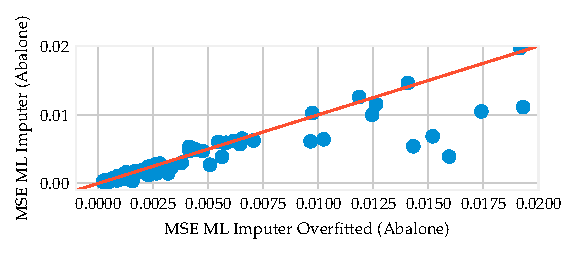
\includegraphics[width=\textwidth]{../figures/abalone/mse_ml_overfit.pdf}
     \caption{Overtrained models are compared with conventionally trained models on the Abalone dataset. Continuous RHSs were imputed to get MSEs.}
     \label{fig:mse-ml-overfit-abalone}
\end{figure}
When continuous data is imputed, ML Imputer uses another network design than when performing a classification task.~\cite[p.~2025]{BIE18}
The behavior regarding overfitting of the numerical regression loss function used in training to generate models to impute continuous data is represented in figure~\ref{fig:mse-ml-overfit-abalone}.
Note that, while in figure~\ref{fig:f1-ml-overfit-adult} a greater score indicates a better performance, in figure~\ref{fig:mse-ml-overfit-abalone} the inverse is true.

It can be observed that the network design used for regression on continuous data is more vulnerable to overfitting than the network used to impute classifiable data.
The majority of cFDs results in nearly equally big MSEs of overfitted models and conventionally trained models.
This is represented in figure~\ref{fig:mse-ml-overfit-abalone} by data points that are positioned in close proximity of the graph of the identity function.

However, a considerable number of data points indicate that the overfitted models perform \( worse \) than the conventionally trained ones.
At first glance, this result appears to be counterintuitive.
One would expect a smaller MSE if more data is used in training.

\begin{figure}[ht]
     \centering
     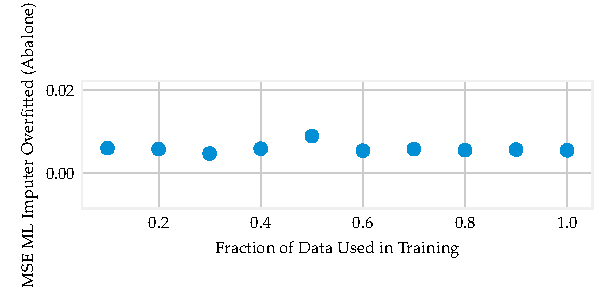
\includegraphics[width=\textwidth]{../figures/abalone/mse-ml-overfitted-fractions.pdf}
     \caption{Overfitted imputation-models are trained with FD \( [2, 3, 6, 7] \rightarrow 5\) on the Abalone dataset with varying dataset-size.}
     \label{fig:mse-ml-overfit-fractions}
 \end{figure}

However, this phenomenon is well-known in practice.
For example, Meng and Xie discuss the effect of training models with differently sized datasets.
They show that more data during training does not necessarily imply a better model.~\cite[p.~1]{MEN14}
On one side, additional data only leads to better models if it provides additional information to solve a problem.
On the other side, as discussed previously, a neural network needs to be sufficiently complex to be able to leverage new data.

Figure~\ref{fig:mse-ml-overfit-fractions} shows the MSE achieved by an overfitted ML Imputer model trained with different fractions of the total dataset.
One can observe that the model trained on 10\% of the total dataset scores a lower MSE as the model trained on 50\% of the total dataset.
Thus, when an overfitted model in figure~\ref{fig:mse-ml-overfit-abalone} performs worse than the conventionally trained counterpart, it can be anticipated that either the additional data contains no or little additional information regarding the regression problem, or that the design of the regression network does not provide enough complexity to incorporate additional information.


\subsection{Dependency detection}
DepDetector is run on number of datasets to detect generalized imputation dependencies.
Since the models used by DepDetector to find minimal dependencies are results of stochastic processes, they are subjects to fluctuations.
To further investigate how these fluctuations influence the result of the DepDetector algorithm, the number of training cycles used in training is varied and performance measures are compared in a section called \emph{stability analysis}.

\subsubsection{DepDetector Results on Various Datasets}
Dependencies were detected on the eight datasets analyzed throughout this work.
Models used by DepDetector were trained on a CPU.
The machine on which the experiment is conducted is equipped with 7.2 GiB of RAM and an Intel Core i5-6300U CPU, a processing unit that runs four cores with clock speeds of 2.40GHz each.
\begin{table}[ht]
    \centering
    \begin{tabular}{lrrrrrr}
        \toprule
        \toprule
        & & & & \multicolumn{1}{c}{Greedy} & \multicolumn{1}{c}{Complete} \\
        Dataset & Cols & Rows & \# FDs & dependencies & dependencies \\
        \midrule
        Abalone & 10 & 4177 & 175 & 7~(42~min) & TL \\
        Adult & 16 & 32561 & 93 & TL & TL \\
        Balance-Scale & 6 & 625 & 7 & 3~(67~s) & 3~(80~s) \\
        Chess & 8 & 28056 & 9 & 1~(117~min) & 1~(340~min) \\
        Iris & 6 & 150 & 9 & 5~(38~s) & 8~(43s) \\
        Letter & 18 & 20000 & 78 & TL & TL \\
        Nursery & 11 & 12960 & 11 & 3~(110~min) & TL \\
        \bottomrule
        \bottomrule
    \end{tabular}
    \caption{Result of running dependency detection on selected datasets. Values in brackets are the runtime until convergence. `TL' indicates that a time limit of 350~min is reached.}\label{tab:dep-detector-performance}
\end{table}
Table~\ref{tab:dep-detector-performance} lists the results.
The column named `Greedy dependencies' numbers how many minimal dependencies were discovered using the greedy search-strategy.
Column `Complete dependencies' indicates how many minimal dependencies were detected using the complete search-strategy.

For six of the eight datasets, the greedy search-strategy converged within 350 minutes.
The complete search-strategy converged for three datasets within 350 minutes.
The complexity of FD discovery is known to be \(\mathcal{O}(n^2(\frac{m}{2})^2 2^m)\), where \( m \) is the number of attributes and \( n \) is the number of records.~\cite[p.~2]{PAP15}
The findings in table~\ref{tab:dep-detector-performance} appear to be according to this rule, since the time limit was reached only for datasets with a great number of columns and/or rows.

\subsubsection{Dependency stability}
To investigate the stability of detected minimal dependencies, DepDetector is run for a fixed RHS with varying numbers of training cycles \( \tau \).
The experiment was conducted on the Iris dataset and the Balance-Scale dataset.
Minimal dependencies were searched following the `complete' search-strategy.

The number of training cycles \( \tau \) is increased stepwise from \( 3 \text{ to } 15 \).
For each \( \tau \) the number of undetected minimal LHSs is calculated.
This is done by first selecting the result of the run with \( \tau_{max} = 15 \) training cycles as a reference.
Then, the LHSs obtained when \( \tau < \tau_{max} \) are compared to the ones obtained when \( \tau = \tau_{max} \).
For each LHS found when DepDetector is run with \( \tau_{max} \) training-cycles that is not contained in the result of a run where \( \tau < \tau_{max} \), the number of undetected minimal LHSs is increased by one.

\begin{figure}[ht]
     \centering
     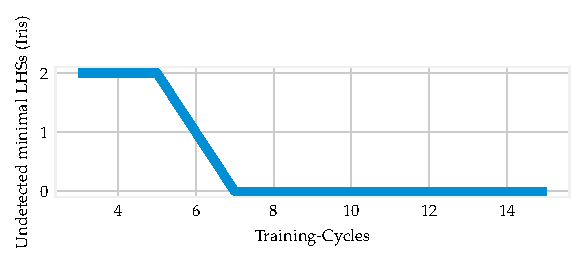
\includegraphics[width=\textwidth]{../figures/iris/dep_detector_lhs_stability}
     \caption{Analysis on the Iris dataset reveals that results become continuously more stable for larger \( \tau \).}
     \label{fig:dep_detector_lhs_stability_iris}
\end{figure}

Figure~\ref{fig:dep_detector_lhs_stability_iris} shows the result of this procedure on the Iris dataset.
When dependencies are searched with \( \tau_{max} \) training cycles, DepDetector finds two minimal LHS combinations and thus two Dependencies.
If \( \tau \in [3, 5] \), both minimal dependencies remained undetected.
In the run where \( \tau = 6 \), one of the two minimal LHSs was found.
For \( \tau \in [7, 15] \) training cycles, DepDetector discovered both minimal dependencies.

There are no fluctuations in the amount of undetected minimal LHSs once seven or more training cycles were used in dependency detection.
This indicates that the minimal dependencies detected by DepDetector do not fluctuate every time new models are trained during detection.

The experiment is repeated on the Balance-Scale dataset.
Figure~\ref{fig:dep_detector_lhs_stability_balance_scale} displays a non-linear behavior when detecting minimal LHSs in function of \( \tau \).
Even though the result obtained for \( \tau = 3 \) is minimal, the result found when \( \tau = 4 \) misses one minimal dependency.
\begin{figure}[ht]
     \centering
     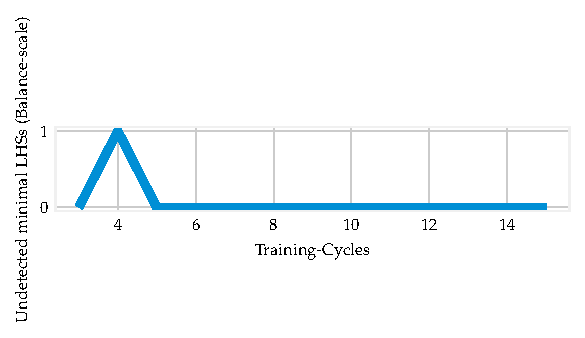
\includegraphics[width=\textwidth]{../figures/balance-scale/dep_detector_lhs_stability.pdf}
     \caption{On the dataset Balance-scale, the analysis of the result shows a peak at \( \tau = 4 \).}
     \label{fig:dep_detector_lhs_stability_balance_scale}
\end{figure}
For all DepDetector-runs performed with five or more training-cycles, all minimal LHSs are detected.
This is another hint that minimal dependencies identified with DepDetector converge to a stable solution.

While these two examples are no proof that DepDetector always yields a stable set of minimal LHSs, they motivate a default value of \( \tau = 10 \) training-cycles during dependency detection.
